\subsection{Measurements of the three parallelisation implementations}

We have compared three different parallelisation implementation: (i)
an R-side parallelism which uses a \texttt{mclapply} call from the R
\texttt{parallel} package. (ii) a first naive openMP implementation
which use \texttt{\#pragma omp critical} around the map-reduce
step. (iii) A re-implementation of the map-reduce step which enabled
that part to be run without the use of \texttt{\#pragma omp critical}.
\begin{figure}[!htbp] \centering
  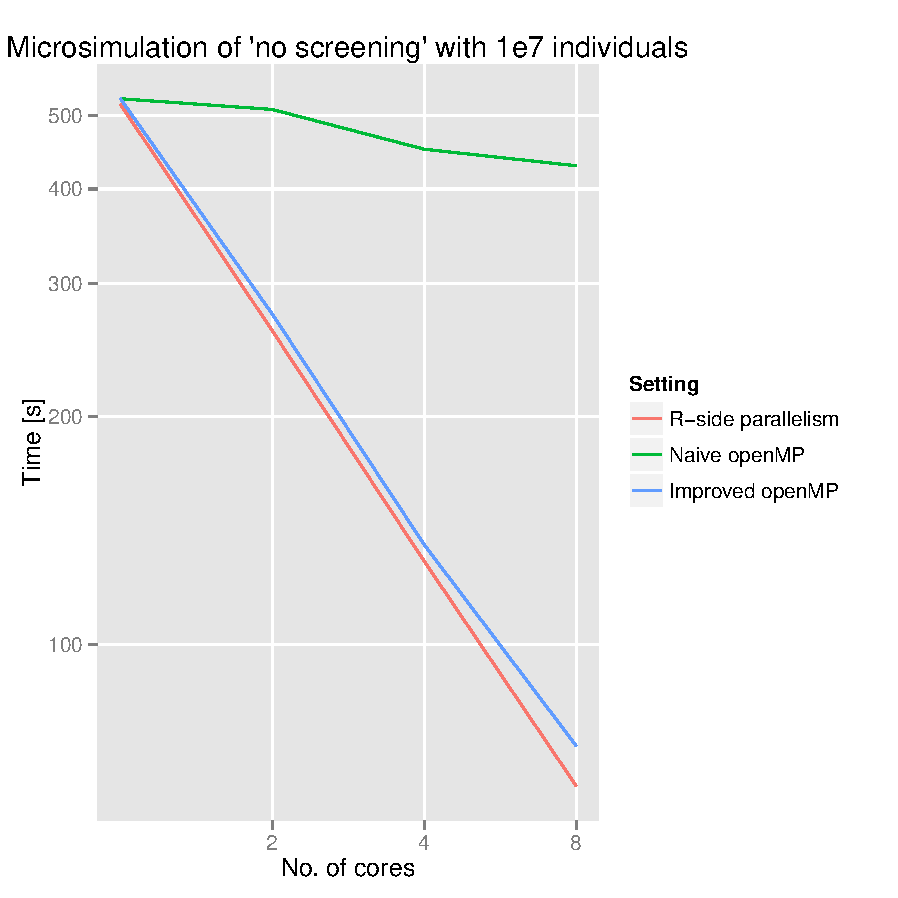
\includegraphics[height=0.5\textheight]{images/implementationProfiling.pdf}
  \caption{implementations...}
  \label{fig:implScaling}
\end{figure} 

Figure \ref{fig:implScaling} shows how the three
different implementations of parallelisation scales with additional
cores. The \emph{R-side parallelism} and \emph{Improved openMP} scales
well with comparable results. The \emph{Naive openMP} implementation
with the \emph{EventReport} mentioned in \ref{fig:cppMot} within
\emph{\#pragma omp critical} statements.



%%% Local Variables: 
%%% mode: latex 
%%% TeX-master: "report" 
%%% End:
